%%%%%%%%%%%%%%%%%%%%%%%%%%%%%%%%%%%%%%%%%%%%%%%%%%%%%%%%%%%%%%%%%%%
% 
% $Id: sec4.tex,v 1.1.1.1 2002/01/02 19:36:28 phil Exp $
%
% $Log: sec4.tex,v $
% Revision 1.1.1.1  2002/01/02 19:36:28  phil
% initial import into CVS
%
% Revision 1.9  1997/08/29 20:06:09  allen
% *** empty log message ***
%
% Revision 1.8  1997/08/28 16:38:36  cguo
% *** empty log message ***
%
% Revision 1.7  1996/08/13 17:10:56  cguo
% *** empty log message ***
%
% Revision 1.6  1996/08/13 00:56:12  cguo
% glossary a problem
%
% Revision 1.5  1996/08/12 23:24:55  cguo
% ready for phil
%
% Revision 1.4  1996/08/06 21:39:12  cguo
% *** empty log message ***
%
% Revision 1.3  1996/04/29 19:03:05  stockie
% ready for carmen
%
% Revision 1.2  1995/08/14  22:18:20  stockie
% - add glossary definitions
% - change labels to depend on lab #
% - use new versions of \quiz, \demo, \technicalnote, etc.
% - add comments to figures
% - elaborate a bit on interpolation methods
%
% Revision 1.1  1995/07/18  21:38:58  stockie
% Initial revision
%
%
%%%%%%%%%%%%%%%%%%%%%%%%%%%%%%%%%%%%%%%%%%%%%%%%%%%%%%%%%%%%%%%%%%%

\section{Discretization}

When computing analytical solutions to differential equations, we are
dealing with \emph{continuous functions}; \ie functions that depend
continuously on the independent variables.  A computer, however, has
only finite storage capacity, and hence there is no way to represent
continuous data, except approximately as a sequence of \emph{discrete}
values.

\begin{example}
  We already saw an example of a discrete function in
  Example~\ref{lab1:exm:conduction-nonlinear}, where the rate function
  $\lambda$, depended on the temperature.
  If $\lambda$ is not known by
  some empirical formula, then it can only be determined by
  experimental  
  measurements at a discrete set of temperature values. 
  In Figure~\ref{lab1:fig:table}, $\lambda$ is given at a sequence of six
  temperature 
  points ( $(T_i, \lambda_i)$, for $i = 0, 1, \dots, 5)$ ), and so is
  an example of a \emph{discrete function}.

  The process of interpolation, which was introduced in
  Example~\ref{lab1:exm:conduction-nonlinear}, will be considered in more
  detail next.
\end{example}

\begin{example}
  Consider the two continuous functions 
  \[
    f(x)=x^3-5x \;\; {\rm and} \;\; g(x)=x^{2/3} . 
  \]
  (In fact, $g(x)$ was the function used to generate the values
  $\lambda(T)$ in Example~\ref{lab1:exm:conduction-nonlinear}.)

  The representation of functions using mathematical notation or
  graphs is very convenient for mathematicians, where continuous
  functions make sense.  However, a computer has a limited storage
  capacity, and so it can represent a function only at a finite number
  of discrete points $(x,y)$.

  One question that arises immediately is: \emph{What do we do if we
    have to determine a value of the function which is not at one of
    the discrete points?}  
  The answer to this question is to use some form of {\em
    interpolation} -- namely 
  to use an approximation procedure to estimate values of the function
  at points between the known values.
%%%%%%%%%%%%
\begin{latexonly}
  \gloss{interpolation}{a method for estimating the value of a
    function at points intermediate to those where its values are
    known.}
  \gloss{forward difference discretization}{used to calculate a
derivative -- uses the current points and points with larger 
independent variable.}
\end{latexonly}
%%%%%%%%%%%%

  For example, linear interpolation approximates the function at
  intermediate points using the straight line segment joining the two
  neighbouring discrete points.
  There are other types of interpolation schemes that are more
  complicated, a few of which are:
  \begin{itemize}
  \item quadratic interpolation: every two sucessive points are joined
    by a quadratic polynomial.
  \item cubic splines: each pair of points is joined by a cubic
    polynomial so that the function values and first derivatives match
    at each point.
  \item Fourier series: instead of polynomials, uses a sum of 
    $\sin nx$ and $\cos nx$ to approximate the function (Fourier
    series are useful in analysis, as well as spectral methods).
  \item Chebyshev polynomials: another type of polynomial
    approximation which is useful for spectral methods.
  \item \dots many others \dots 
  \end{itemize}
  For details on any of these interpolation schemes, see a numerical
  analysis text such as that by \cite{burden-faires}.   

  An application of linear interpolation to  discrete versions of
  the functions $f$ and $g$ is shown in
  Figure~\ref{lab1:fig:discrete-f}.
  \begin{figure}[htbp]
    \begin{center}
      \leavevmode
%%%%%%%%%%%%%%%%%%%%%%%%%%%%%%%%%%%%%%%%%%%%%%%%%%%%%
%  NOTE: These plots were created using the 
%  Gnuplot script ``discrete/genplots.gin''.  
%%%%%%%%%%%%%%%%%%%%%%%%%%%%%%%%%%%%%%%%%%%%%%%%%%%%%
      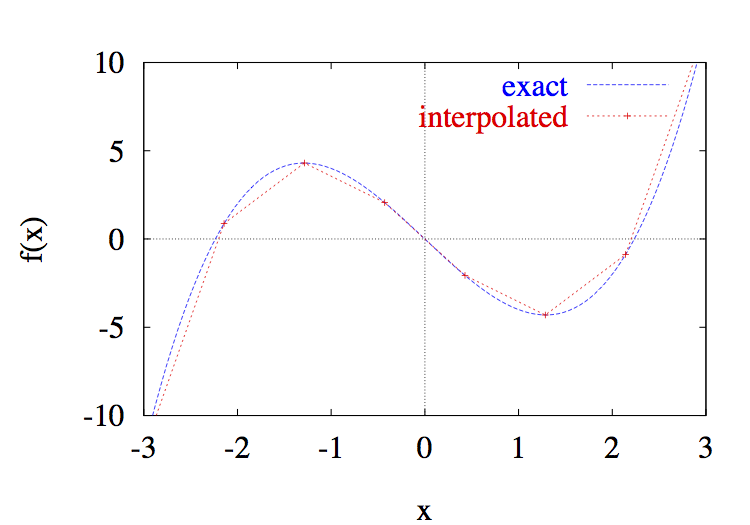
\includegraphics[height=3.5in]{discrete/f}
      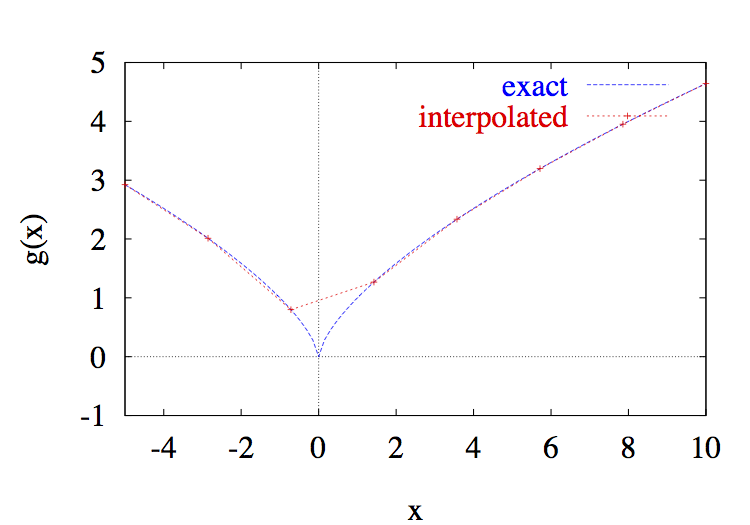
\includegraphics[height=3.5in]{discrete/g}
      \caption{The functions $f$ and $g$ are known only at discrete
        points.  The function can be approximated at other values by
        linear interpolation, where straight line segments are used
        to join successive points.}
      \label{lab1:fig:discrete-f}
    \end{center}
  \end{figure}

  Depending on the function, or number of location of the points
  chosen, the approximation may be more or less accurate.  In
  Figure~\ref{lab1:fig:discrete-f}, it is not clear which function is
  approximated more accurately.  In the graph of $f(x)$, the error
  seems to be fairly small throughout.  However, for the function
  $g(x)$, the error is large near $x=0$, and then very small
  elsewhere.  
  This problem of \emph{accuracy} of
  discrete approximations will come up again and again in this course.

%%%%%%%%%%%%
  \demo{discrete.cgi}{Here is an interactive example demonstrating the use of interpolation (linear and cubic) in approximating functions.\label{lab1:demo:discrete}}   

%\technicalnote{Details on how the interpolation example works \dots}{See Appendix }{ for details on how the interpolation example works.}{lab1:tech:discrete}  

%%%%%%%%%%%%

%%%%%%%%%%%%
  \quiz{quiz-interp.html}{After you finish the interpolation exercise, try out this short quiz.}
%%%%%%%%%%%%
\end{example}

%%%%%%%%%%%%%%%%%%%
\begin{latexonly}
\gloss{grid}{when referring to discretization of a DE, a grid is a set
  of discrete values of the independent variables, defining a {\em
    mesh} or array of points, at which the solution is approximated.}
\end{latexonly}
%%%%%%%%%%%%%%%%%%%
When solving differential equations numerically, it is essential to
reduce the continuous problem to a discrete one.
The basic idea is to look for an 
approximate solution, which is defined at a finite number of 
discrete points.
This set of points is called a \emph{grid}.
Consider the one-dimensional conduction problem of
Example~\ref{lab1:exm:conduction}, which in its most general form reads  
\begin{equation}
  \frac{dT}{dt} = -\lambda(T,t) \, (T-T_a),
  \label{lab1:eq:conduction}
\end{equation}
with initial temperature $T(0)$.  

When we say we want to design a numerical procedure for solving
this initial value problem, what we want is a procedure for
constructing a sequence of approximations,
\[
T_0, \, T_1, \, \ldots, \, T_i, \, \ldots,
\]
defined at a set of discrete $t$-points, 
\[
t_0<t_1<\cdots<t_i<\cdots.
\]
Each $T_i$ is an approximation of the actual temperature at $t_i$;
that is
\[
T_i \approx T(t_i).
\]
For now, we will consider equally-spaced points, each of which is
separated by a distance \dt, so that 
\[
t_i=t_0+i \dt .
\]
An example of
such a grid is shown in Figure~\ref{lab1:fig:discrete-points}.
\begin{figure}[htbp]
  \begin{center}
    \setlength{\unitlength}{4pt}
    \leavevmode
    {\large
    \begin{picture}(100,20)(0,10)
        \put(0,20){ \vector(1,0){90} }
        \put(93,19){$t$}
        \put(15,14){$t_0$}
        \put(15,20){ \circle*{1} }
        \put(25,14){$t_1$}
        \put(25,20){ \circle*{1} }
        \put(35,14){$t_2$}
        \put(35,20){ \circle*{1} }
        \put(45,20){ \circle*{1} }
        \put(49,14){$\cdots$}
        \put(55,20){ \circle*{1} }
        \put(65,14){$t_i$}
        \put(65,20){ \circle*{1} }
        \put(75,20){ \circle*{1} }
        \put(79,14){$\cdots$}
        \put(16,22.5){\vector(1,0){10}}
        \put(26,22.5){\vector(-1,0){10}}
        \put(19,24){\dt}
    \end{picture}
    }
    \caption{A grid of equally-spaced points, $t_i=t_0+i\dt$, for
      $i=0,1,2,\ldots$} 
    \label{lab1:fig:discrete-points}
  \end{center}
\end{figure}

This process of reducing a continuous problem to one in a finite number
of discrete unknowns is called \emph{discretization}.
The actual mechanics of discretizing differential equations are
introduced in the following section.
%%%%%%%%%%%%%%%%%
\begin{latexonly}
\gloss{discretization}{when referring to DE's, it is the process
  whereby the independent variables 
  are replaced by a \emph{grid} of discrete points; the dependent
  variables are replaced by approximations at the grid points; and the
  derivatives appearing in the problem are replaced by a \emph{finite
    difference} approximation.  The discretization process replaces
  the DE (or DE's) with an algebraic equation or finite system of
  algebraic equations which can be solved on a computer.}
\end{latexonly}
%%%%%%%%%%%%%%%%%

\quiz{quiz1.html}{Here is a short quiz on discretization.}

\paragraph{Summary}

The basic idea in this section is that continuous functions can be
approximated by discrete ones, through the process of {\em
  discretization}.  
In the course of looking at discrete
approximations in the interactive example, we introduced the idea of the
\emph{accuracy} of an approximation, and showed that increasing the
accuracy of an approximation is not straightforward.

We introduced the notation for approximate solutions to differential
equations on a grid of points.  The mechanics of discretization as
they apply to differential equations, will be investigated further in the remainder of
this Lab, as well as in \htmladdnormallink{Lab~\#2}{\LabtwoURL}.




%%% Local Variables: 
%%% mode: latex
%%% TeX-master: "lab1"
%%% End: 
